\documentclass[12pt]{article}
\usepackage[margin=1in]{geometry}
\usepackage{graphicx,float}
\usepackage{amsmath,amssymb,booktabs,array,enumitem,setspace,hyperref}
\hypersetup{colorlinks=true,urlcolor=black,linkcolor=black}
\onehalfspacing
\setlength{\parindent}{2.75em}
\setlist[enumerate,1]{leftmargin=*,itemsep=1.5ex}
\setlist[enumerate,2]{leftmargin=*,itemsep=1ex}
\begin{document}
\begin{center}
\large\textbf{ECON 344: Economics of Crime \\ Midterm Review: Research Designs and Mechanisms}
\end{center}
\medskip
\noindent\textbf{Instructions:} Answer each part in two to four sentences unless a calculation is requested. No prior reading of the papers is necessary: the relevant background is provided below. 


\section*{Section 1: Cognitive Behavioral Therapy and Crime in Liberia}
\noindent \textit{Reference:} Blattman, Christopher, Julian C. Jamison, and Margaret Sheridan (2017), 
``Reducing Crime and Violence: Experimental Evidence from Cognitive Behavioral Therapy in Liberia,'' \emph{American Economic Review}.
\\
\noindent \textbf{Study:} Blattman, Jamison, and Sheridan recruited men in Liberia who were involved in crime or other high-risk activities.
They studied an eight-week cognitive behavioral therapy (CBT) program designed to improve self-control, patience, and the ability to adopt a noncriminal lifestyle.
Independently, participants could also receive a \$200 cash grant.
Random assignment generated four groups: neither intervention, CBT only, cash only, and both CBT and cash.
In the original study, CBT alone and cash alone reduced crime and violence in the short run, but their impacts faded;
the combination produced more persistent reductions over the following year.

\begin{enumerate}

\item Why do you think CBT would reduce criminal behavior? What is the hypothesized mechanism?
% SOLUTION:
% CBT may improve self-control, patience, emotion regulation, and
% nonviolent conflict resolution. These changes could reduce impulsive
% offending and make noncriminal choices more attractive or feasible.
% This is a hypothesized behavioral mechanism rather than a claim that
% the experiment separately identifies each channel.
\vspace{3cm}

\item Imagine that, instead of randomly assigning therapy, the researchers compared men who voluntarily attended CBT with men who did not. Would a difference in subsequent criminal behavior establish that CBT caused the difference? Explain a specific source of selection bias and the direction.
% SOLUTION:
% No. Individuals who voluntarily participate in CBT may differ from
% nonparticipants in characteristics that also affect criminal behavior.
% For example, more motivated men may be more likely to attend CBT and
% less likely to commit crimes even without treatment. This would bias
% the estimated effect downward (making CBT appear more effective).
% Alternatively, individuals at particularly high risk of crime may be
% more likely to seek treatment, potentially biasing the estimated
% effect upward. The direction depends on the selection mechanism.
\vspace{10ex}

\item Why does random assignment make the comparison between the CBT and non-CBT groups more credible? Is it necessary for the groups to have identical crime rates \emph{in the realized sample} before treatment?
% SOLUTION:
% Random assignment makes treatment status independent of potential
% outcomes in expectation, so systematic pre-existing differences
% should not drive average differences in outcomes across groups.
% The groups need not have identical baseline crime rates in the
% realized sample: random imbalances can occur by chance.
% Randomization provides comparability in expectation, not exact
% balance in every realized experiment.
\vspace{4cm}


\item What does this table show that helps support the credibility of the randomization? What would you look for in a table like this?
\begin{figure}[H]
\centering
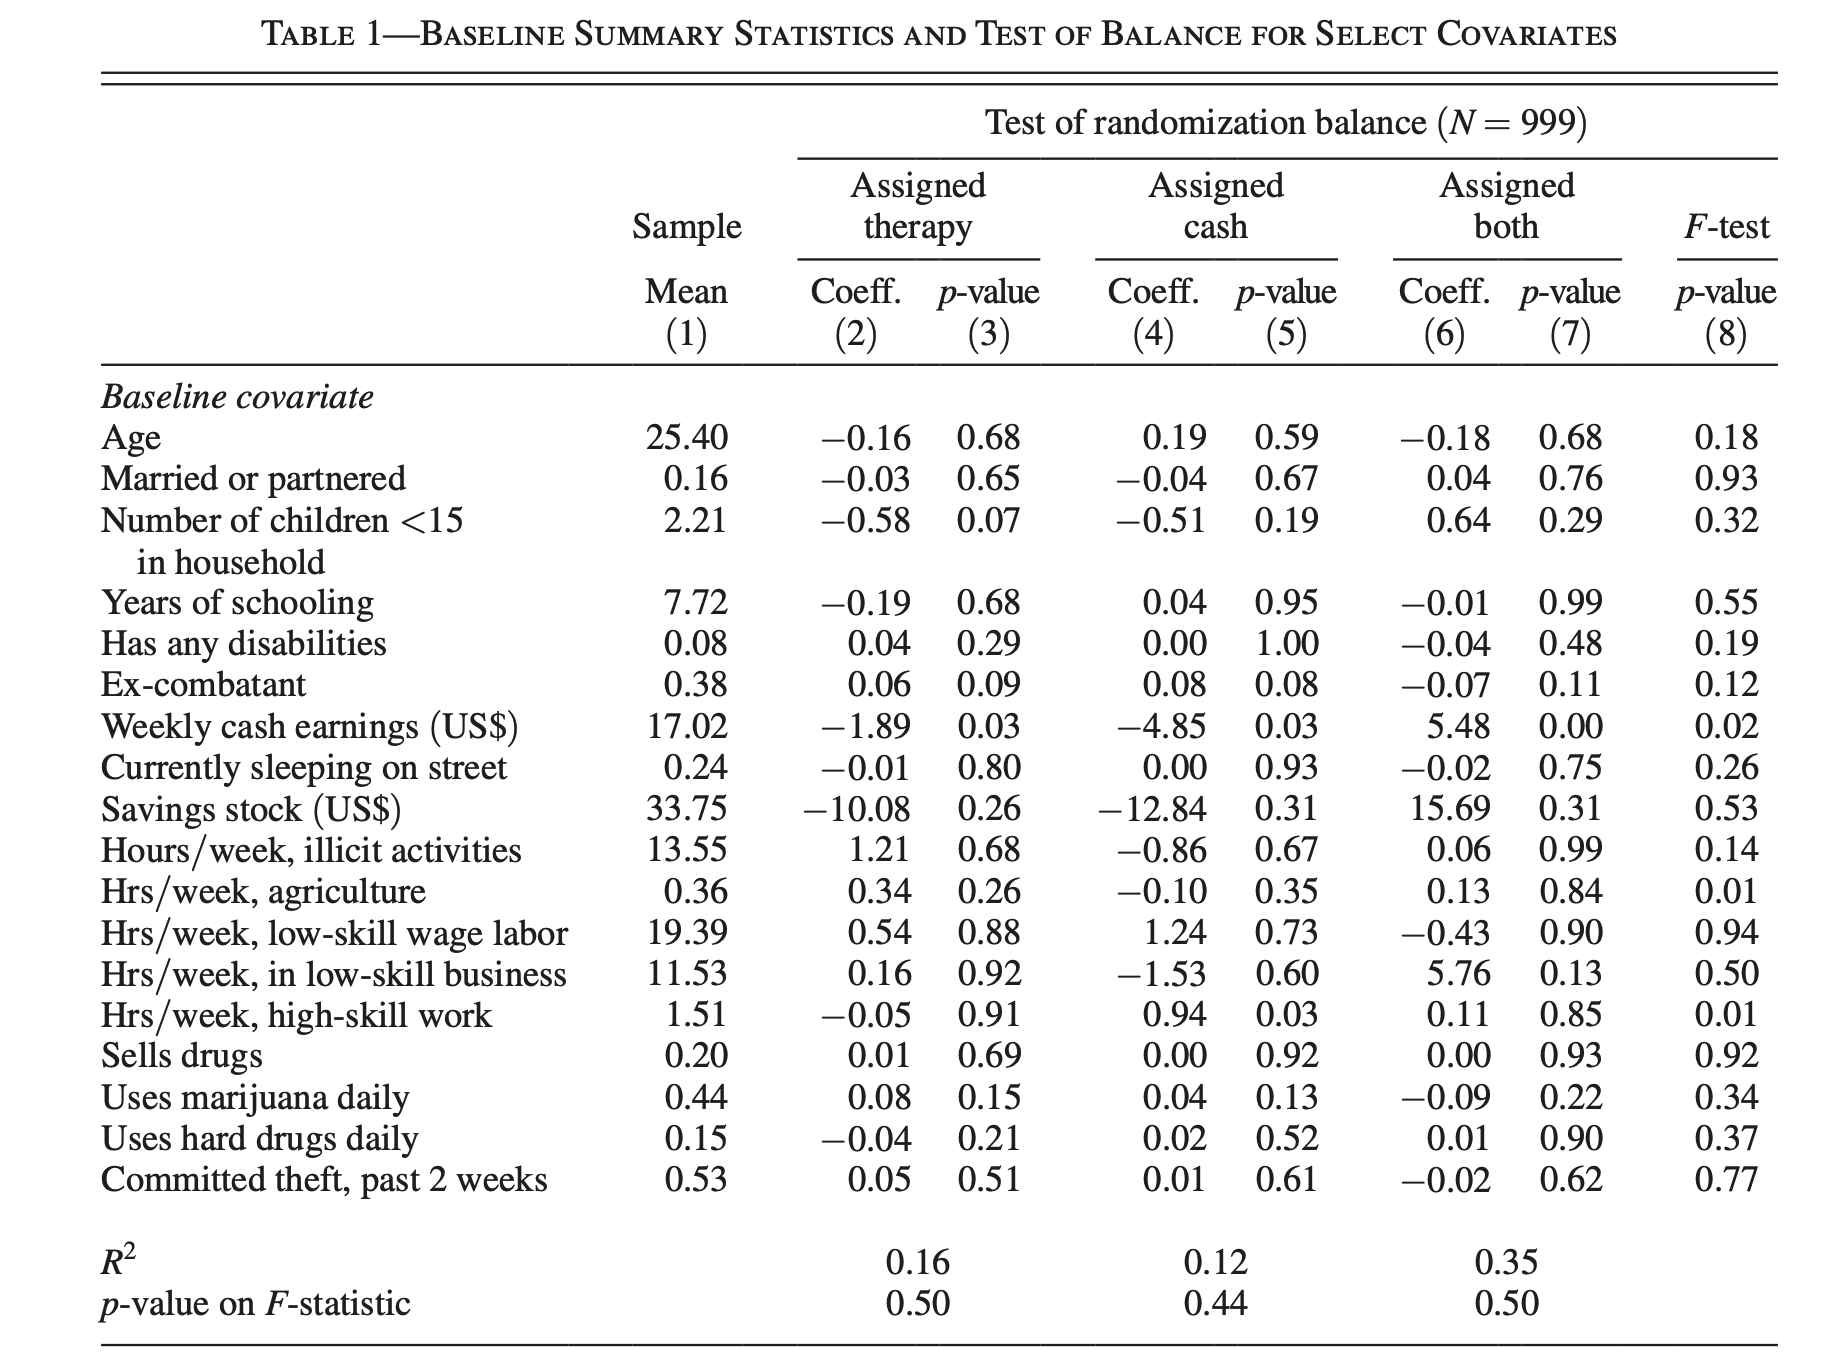
\includegraphics[width=0.95\textwidth]{balance.png}
\end{figure}

% SOLUTION:
% This table tests whether participants assigned to different
% treatment groups had similar characteristics before treatment.
% Since treatment was randomly assigned, we expect the groups
% to be balanced on average, although some differences can arise
% by chance in a finite sample.
%
% We would look at:
% (1) Whether the coefficients on treatment assignment are close
%     to zero, indicating small baseline differences.
% (2) Whether the p-values are statistically significant.
% (3) Whether there are systematic differences across many
%     predetermined characteristics.
% (4) The F-tests, which test whether a baseline characteristic
%     differs jointly across treatment groups.
%
% In this table, most baseline characteristics appear balanced.
% For example, age, years of schooling, and prior theft do not
% differ significantly across the treatment groups.
%
% However, there are some statistically significant differences.
% Weekly cash earnings differ across treatment groups
% (F-test p-value = 0.02), as do hours in agriculture and
% high-skill work (both F-test p-values = 0.01).
% These differences could arise by chance under randomization.
%
% The bottom row reports joint tests of whether baseline
% characteristics predict assignment to each treatment arm.
% The p-values are 0.50, 0.44, and 0.50, so we fail to reject
% the null that these characteristics jointly have no
% predictive power for treatment assignment.
%
% Overall, the table is broadly consistent with successful
% randomization, although it does not prove that randomization
% was implemented perfectly.
%
% Importantly, statistically insignificant differences do not
% mean the groups are exactly identical, and a few significant
% differences do not automatically invalidate an RCT.

\vspace{4cm}


\item Consider this regression, where $Y_i$ is an indicator equal to one if participant $i$ commits a crime during follow-up:
\[
Y_i=\alpha+\beta\,CBT_i+\gamma\,Cash_i+\delta(CBT_i\times Cash_i)+\varepsilon_i.
\]
\begin{enumerate}
\item Is this a simple OLS regression? Why or why not?
\vspace{2cm}
% SOLUTION:
% The equation can be estimated using OLS, even though the dependent
% variable is binary. This is a linear probability model (LPM).
% Because it includes two treatment indicators and an interaction,
% it is a multiple regression rather than simple (bivariate) OLS.
% The random assignment of the interventions, not OLS itself,
% supports a causal interpretation of the treatment coefficients.

\item What does $\alpha$ represent? Interpret $\beta$, $\gamma$, and $\delta$.
\vspace{4cm}
% SOLUTION:
% alpha: Probability of crime for the control group receiving neither.
% beta: Effect of CBT among individuals who do not receive cash.
% gamma: Effect of cash among individuals who do not receive CBT.
% delta: Additional effect of combining CBT and cash beyond the sum
% of their separate effects (the interaction effect).
% Since Y is binary, coefficients represent changes in probability.
% Multiplying by 100 converts these to percentage points.

\item Write the expected probability of crime for each of the four treatment groups.
\vspace{4cm}
% SOLUTION:
% Neither:      E[Y|CBT=0,Cash=0] = alpha
% CBT only:     E[Y|CBT=1,Cash=0] = alpha + beta
% Cash only:    E[Y|CBT=0,Cash=1] = alpha + gamma
% CBT and cash: E[Y|CBT=1,Cash=1] = alpha + beta + gamma + delta

\item What is the effect of adding CBT for someone who receives cash? What is the effect of adding cash for someone who receives CBT?
\vspace{4cm}
% SOLUTION:
% Effect of CBT conditional on receiving cash: beta + delta.
% Effect of cash conditional on receiving CBT: gamma + delta.
% The interaction term modifies the effect of one intervention
% depending on whether the other intervention is received.
\end{enumerate}
\vspace{8ex}

\item Here is a table reporting intent-to-treat (ITT) effects for each treatment arm relative to the control group:
\begin{figure}[H]
\centering
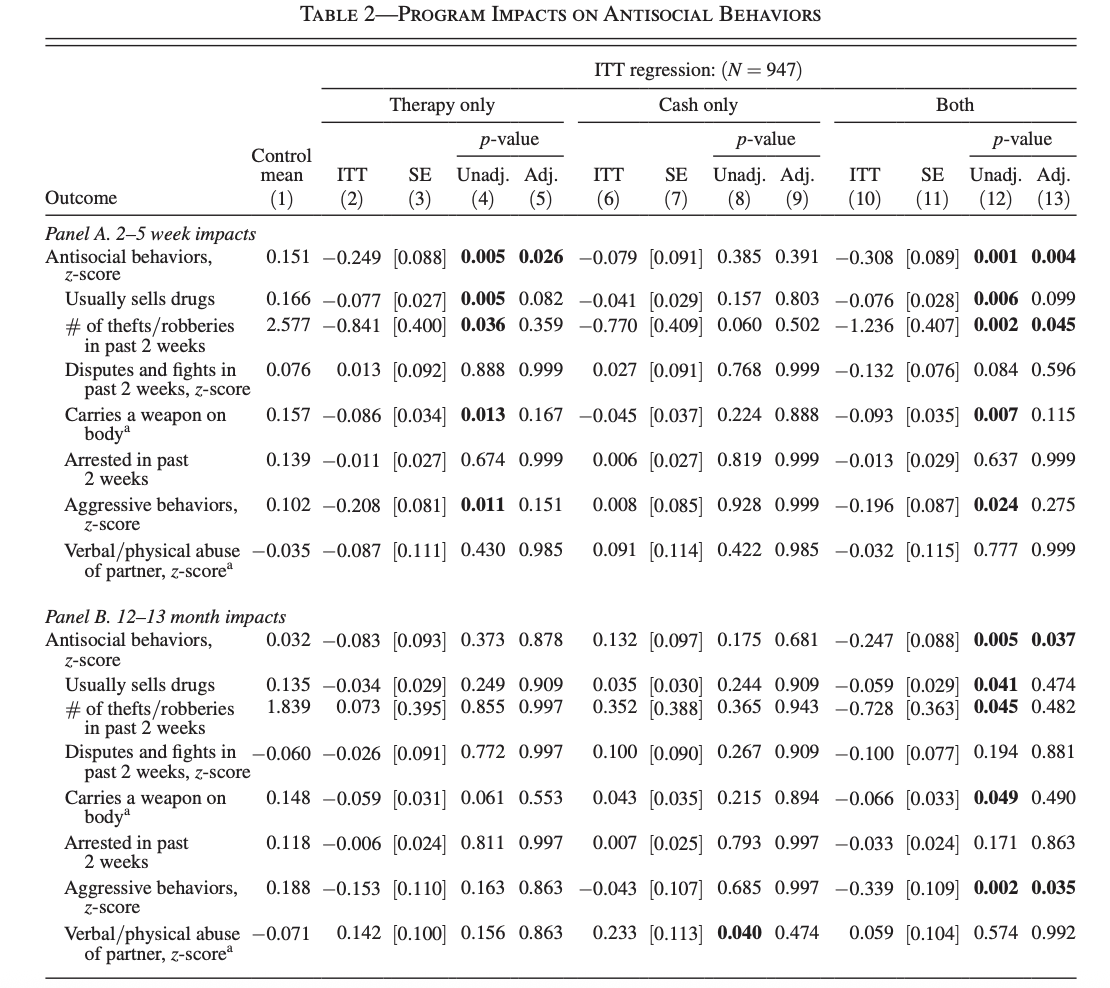
\includegraphics[width=0.95\textwidth]{CBT_table.png}
\end{figure}
\begin{enumerate}
\item Calculate the short-term and long-term predicted probability of being arrested in each treatment arm.
\vspace{4cm}

% SOLUTION:
% The predicted probability of arrest is calculated by adding
% the estimated ITT effect for each treatment arm to the control mean.
% We use the row "Arrested in past 2 weeks."
%
% PANEL A: SHORT-TERM EFFECTS (2-5 weeks)
% Control mean = 0.139
%
% Neither intervention:
% 0.139 = 13.9%
%
% CBT only:
% 0.139 - 0.011 = 0.128 = 12.8%
%
% Cash only:
% 0.139 + 0.006 = 0.145 = 14.5%
%
% CBT and cash:
% 0.139 - 0.013 = 0.126 = 12.6%
%
% PANEL B: LONG-TERM EFFECTS (12-13 months)
% Control mean = 0.118
%
% Neither intervention:
% 0.118 = 11.8%
%
% CBT only:
% 0.118 - 0.006 = 0.112 = 11.2%
%
% Cash only:
% 0.118 + 0.007 = 0.125 = 12.5%
%
% CBT and cash:
% 0.118 - 0.033 = 0.085 = 8.5%
%
% SUMMARY:
%                    Short-term      Long-term
% Control               13.9%           11.8%
% CBT only              12.8%           11.2%
% Cash only             14.5%           12.5%
% CBT + Cash            12.6%            8.5%
%
% These are fitted probabilities obtained by adding each
% treatment arm's ITT estimate to the control mean.
% Note that none of the arrest ITT estimates is statistically
% significant at conventional levels in this table.


\item Relative to neither intervention, by how many \emph{percentage points} does the combined treatment change the probability of arrest?
\vspace{4cm}
% SOLUTION:
% Because the table reports treatment-arm effects relative to the
% control group, we can read the combined-treatment ITT directly.
% Short term: -0.013 = -1.3 percentage points (12.6% vs. 13.9%).
% Long term: -0.033 = -3.3 percentage points (8.5% vs. 11.8%).
% Neither estimate for arrest is statistically significant in the table.
% In the factorial regression, the same contrast equals beta+gamma+delta.

\item Using the estimated effects in the arrest row, calculate the implied interaction between CBT and cash for each follow-up period. A classmate says ``A negative interaction means cash has no effect unless a person gets CBT.'' Is that conclusion correct? Explain.
\vspace{4cm}
% SOLUTION:
% In a factorial regression, the interaction equals the combined-arm
% effect minus the CBT-only effect minus the cash-only effect.
% Short term: -0.013 - (-0.011) - 0.006 = -0.008.
% Long term: -0.033 - (-0.006) - 0.007 = -0.034.
% These are implied point estimates, not separately reported
% interaction coefficients or tests of their significance.
% Cash without CBT has estimated effects of +0.006 (short term)
% and +0.007 (long term) on arrest probability, not zero by assumption.
% The effect of cash with CBT equals the combined-arm effect minus the
% CBT-only effect: -0.002 (short term) and -0.027 (long term).
% A negative interaction means the marginal effect of cash is more
% negative among CBT recipients, not that cash has zero effect otherwise.
\end{enumerate}
\vspace{8ex}

\item One possible explanation for the persistent effect of combining CBT and cash is that the money lets participants spend more time practicing new behaviors and investing in a different lifestyle. Suggest one additional outcome the researchers could measure to distinguish this explanation from the simpler hypothesis that cash temporarily raises legal income and thereby reduces incentives for crime.
\vspace{4cm}
% SOLUTION:
% One outcome is continued use of CBT-related behaviors or skills,
% such as self-control, conflict resolution, or avoidance of risky peers.
% If participants receiving CBT and cash maintain these behaviors
% after the grant has been spent, this would be consistent with
% cash helping reinforce lasting behavioral changes.
% Alternatively, researchers could measure legal employment,
% savings, or investments in legitimate income-generating activities.
% These outcomes could help distinguish persistent changes in
% behavior from a temporary income effect.
% However, observing these outcomes would not by itself prove
% that the proposed mechanism is causal.
\vspace{8ex}

\item What are two potential threats to identification in this experiment? Good reminder that even RCTs can have challenges with internal validity!
\vspace{4cm}
% SOLUTION:
% 1. Differential attrition: If treated participants are more or
% less likely to be located at follow-up, and attrition is related
% to potential criminal outcomes, comparisons among respondents
% may no longer preserve the original randomization.
%
% 2. Spillovers or interference: Treated participants could
% influence untreated participants, for example by changing
% peer behavior or local criminal opportunities. In this case,
% the control group's outcomes may also be affected by treatment,
% complicating the interpretation of the estimated effects.
%
% Other acceptable answers include differential measurement or
% reporting of crime, and noncompliance with assigned treatment
% when interpreting effects of actual participation.
% Noncompliance alone does not invalidate the ITT estimate;
% it changes what the assignment-based comparison identifies.
\vspace{8ex}

\item In the Becker model, an individual compares the expected utility of crime with the utility of not committing crime. Explain one way CBT and a cash grant might change that comparison. Why might a model that only changes the probability of arrest or the size of punishment miss important channels of these interventions?
\vspace{4cm}
% SOLUTION:
% CBT may improve self-control, patience, or decision-making,
% changing how individuals evaluate immediate rewards from crime
% relative to future costs and benefits. It may also change the
% psychological payoff from criminal behavior.
%
% A cash grant may increase resources available for legitimate
% economic activities, making noncriminal options more attractive.
% It may also relax credit constraints, allowing individuals to
% invest in employment or self-employment opportunities.
%
% Neither intervention necessarily changes the objective probability
% of apprehension or the formal punishment for crime. A framework
% focused only on arrest probabilities and penalties would miss
% changes in preferences, behavioral skills, liquidity constraints,
% and the returns to legitimate economic opportunities.
\end{enumerate}
\clearpage

\section*{Section 2: Close Elections, Drug Trafficking, and Violence in Mexico}
\noindent \textit{Reference:} Dell, Melissa (2015), ``Trafficking Networks and the Mexican Drug War,'' \emph{American Economic Review}.
\\
\noindent \textbf{Study:} During Mexico's campaign against drug trafficking, mayors from the National Action Party (PAN) were more likely to cooperate with federal anti-drug enforcement.
Dell studies municipalities where a PAN mayoral candidate narrowly won or narrowly lost an election.
She compares subsequent drug-related violence across these close elections using a regression discontinuity design (RDD).
The study finds that close PAN victories increased drug-related violence locally.
It also provides evidence that enforcement can redirect trafficking through other routes, affecting violence elsewhere.

\begin{enumerate}
\item Define the running variable as $X_i=$ PAN's vote share minus its strongest opponent's vote share, in percentage points. Explain:
\begin{enumerate}
\item What is the cutoff? Which municipalities are treated and which are the comparison group?
\vspace{1.8cm}
% SOLUTION:
% The cutoff is X_i = 0, where PAN and its strongest opponent have
% equal vote shares. Municipalities just above zero (PAN barely wins)
% are treated; those just below zero (PAN barely loses) are controls.
\item Why might comparing a municipality where PAN wins by 0.2 percentage points with one where PAN loses by 0.2 points be more credible than comparing all PAN and non-PAN municipalities?
\vspace{1.8cm}
% SOLUTION:
% Very close winners and losers are plausibly similar in their observed
% and unobserved determinants of future violence. Across all elections,
% PAN and non-PAN municipalities could differ systematically in voter
% preferences, economic conditions, pre-existing violence, etc.
% Near the threshold, a tiny difference in votes changes who governs.
\item What assumption is required for a causal interpretation? State it in your own words.
\vspace{1.8cm}
% SOLUTION:
% In the absence of a PAN victory, municipalities that barely elect PAN
% would have had essentially the same average potential outcomes as
% those where PAN barely loses. Potential outcomes must change smoothly
% through the zero vote-margin cutoff, absent the treatment.
% Precise sorting/manipulation of the close election outcome would
% undermine this assumption; other policies should not jump at zero.
\end{enumerate}
\vspace{8ex}

\item Consider the following local linear RDD regression, where $Y_i$ is the post-election homicide rate (homicides per 100,000 residents), $X_i$ is the PAN victory margin defined above, and $D_i=1\{X_i>0\}$ indicates a PAN win:
\[
Y_i=\alpha+\tau D_i+\beta X_i+\gamma(D_i\times X_i)+\varepsilon_i.
\]
Suppose this equation is estimated using municipalities with elections close to the cutoff.
\begin{enumerate}
\item What do $\alpha$ and $\tau$ represent? Which coefficient is the RDD estimate of the causal effect of electing a PAN mayor?
\vspace{1.8cm}
% SOLUTION:
% alpha is the predicted homicide rate immediately below the cutoff,
% for a municipality where PAN barely loses (X approaches 0 from below).
% tau is the jump in the conditional mean outcome at X=0: the predicted
% rate immediately above minus immediately below zero. It is the sharp
% RDD estimate of the local causal effect of a PAN victory, assuming
% the continuity/no-manipulation conditions hold.
\item What do $\beta$ and $\gamma$ represent? Why might we allow the relationship between election margin and homicide rates to differ on either side of the cutoff?
\vspace{1.8cm}
% SOLUTION:
% beta is the slope of the outcome with respect to the PAN vote margin
% on the losing side (D=0). The slope on the winning side is beta+gamma.
% Allowing different slopes avoids imposing an identical relationship
% between vote margin and homicides to the left and right of zero.
\item Draw an example of a hypothetical RDD graph with a discontinuity at the cutoff. Label the axes, the cutoff, and the estimated treatment effect.
\vspace{1.8cm}
% SOLUTION:
% Horizontal axis: PAN victory margin in percentage points (X_i).
% Vertical axis: homicide rate per 100,000 residents (Y_i).
% Mark the cutoff X_i=0 with a vertical dashed line. Draw fitted
% outcome curves or straight lines separately to the left and right.
% Make their fitted values at zero differ, and label the vertical
% distance between the two fitted limits as tau (the RDD estimate).
% For example, limits of 18 and 24 imply tau=24-18=6, but any
% clear hypothetical discontinuity is acceptable. The left and right
% slopes may differ. The jump, not the slope, is the RDD effect.
\end{enumerate}
\vspace{8ex}

\item Below are the results from the paper.
\begin{figure}[H]
\centering
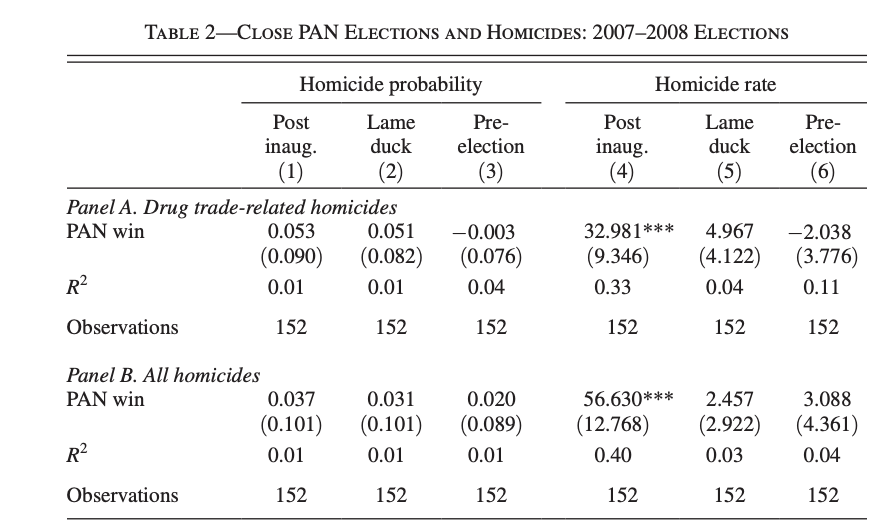
\includegraphics[width=0.95\textwidth]{rdd_table.png}
\end{figure}
\begin{enumerate}
\item Interpret the RDD estimates in columns (1) and (4)
of Panel A. What do the coefficients tell us about the effect
of narrowly electing a PAN mayor on drug trade-related
homicides? Are these effects statistically significant?
\vspace{1.8cm}
% SOLUTION:
% The RDD estimate is the coefficient on "PAN win."
% It measures the discontinuous change in the outcome at the
% electoral cutoff, comparing municipalities where PAN narrowly
% wins with those where PAN narrowly loses.
%
% Panel A: Drug trade-related homicides
% Column (1): Homicide probability, post-inauguration = 0.053.
% This is a 5.3 percentage point increase, but it is not
% statistically significant (SE = 0.090).
%
% Column (4): Homicide rate, post-inauguration = 32.981.
% Narrowly electing a PAN mayor increases the drug trade-related
% homicide rate by approximately 32.98 homicides per 100,000
% residents (in the rate units defined by the paper).
% This estimate is statistically significant at the 1% level.
%
% Panel B: All homicides
% Column (4): Homicide rate, post-inauguration = 56.630.
% Narrowly electing a PAN mayor increases the overall homicide
% rate by approximately 56.63 homicides per 100,000 residents
% (in the rate units defined by the paper).
% This estimate is also statistically significant at the 1% level.
%
% Importantly, these effects are estimated for close elections
% and represent local causal effects at the electoral cutoff,
% under the RDD identifying assumptions.
%
% The estimates for the lame-duck and pre-election periods
% are much smaller and statistically insignificant.
% This is consistent with violence increasing after PAN mayors
% take office, rather than before inauguration.
\item Does this estimate mean that electing a PAN mayor increases homicides by the same amount in \emph{every} Mexican municipality? Why or why not?
\vspace{1.8cm}
% SOLUTION:
% No. The design identifies a local effect for municipalities with
% very close elections at the zero margin, not necessarily for
% municipalities with landslide elections. Effects may vary by local
% trafficking routes, cartel competition, enforcement, or other factors.
\item A student concludes that reducing anti-drug enforcement would necessarily reduce violence everywhere. Does this follow from the estimate? Explain.
\vspace{1.8cm}
% SOLUTION:
% No. The estimate concerns the local causal effect of barely electing
% a PAN mayor, a political change associated with enforcement, not a
% universal effect of all enforcement changes. Lower enforcement need
% not reverse the treatment effect symmetrically; organizational
% responses and violence may vary across places and time. Violence is
% only one of several relevant policy outcomes.
\end{enumerate}
\vspace{8ex}

\item Suppose there is evidence that candidates can precisely manipulate reported vote counts to turn narrow losses into narrow wins. How would this affect the credibility of the RDD? What empirical pattern near the cutoff might alert you to this problem?
\vspace{1.8cm}
% SOLUTION:
% Precise manipulation could make close winners systematically
% different from close losers, invalidating the continuity logic.
% Evidence might include bunching just above zero, a discontinuity
% in the density of the vote margin, or abrupt jumps in predetermined
% municipal characteristics at the cutoff. Such evidence raises doubts;
% density tests alone do not establish or refute validity definitively.
\vspace{8ex}

\item Suppose municipalities on both sides of the cutoff have similar pre-election violence, income, and population. Does this \emph{prove} the RDD is valid? What does checking these variables help establish?
\vspace{1.8cm}
% SOLUTION:
% No. Balance on observed pre-election characteristics is reassuring
% but cannot prove that all unobserved potential-outcome determinants
% are continuous at zero. These checks can reveal suspicious sorting,
% compositional changes, or other discontinuities at the threshold.
\vspace{8ex}

\item Dell argues that crackdowns can weaken an incumbent trafficking organization, giving rival groups an incentive to fight for its territory. Explain why more enforcement could therefore increase measured violence even if it directly disrupts criminal activity. Does increased violence necessarily imply that enforcement has no benefits?
% SOLUTION:
% Enforcement may disrupt a dominant organization and destabilize its
% control of routes, provoking violent competition among rival groups.
% Violence can therefore increase even as some trafficking operations
% are curtailed. Rising homicides do not prove that enforcement has no
% benefits: effects on trafficking, public safety, and longer-run
% outcomes also matter, though violence is an important social cost.
\vspace{8ex}

\item Consider a municipality that lies on an alternative trafficking route, next to a municipality where PAN narrowly wins. 
Traffickers may reroute shipments through the first municipality to avoid stricter enforcement in the second.
\begin{enumerate}
\item Could the first municipality experience a change in violence even if its own mayoral election outcome does not change? Explain.
\vspace{1.8cm}
% SOLUTION:
% Yes. Traffickers may move shipments or contest routes in response to
% neighboring enforcement. That can change violence in the first
% municipality even if its own election outcome is unchanged.
\item Why is this a potential problem when interpreting local treatment effects as the \emph{total} effect of the crackdown? Identify the relevant spillover or interference issue.
\vspace{1.8cm}
% SOLUTION:
% One municipality's election outcome can affect outcomes in another,
% violating the no-interference part of SUTVA. An RDD comparing own
% close-election winners and losers may fail to capture violence
% displaced to other places; even its direct local contrast can be
% contaminated if comparison municipalities are exposed to spillovers.
% The local RDD coefficient should not automatically be interpreted
% as the aggregate or nationwide effect of the enforcement campaign.
\end{enumerate}
\end{enumerate}
\clearpage

\end{document}